% !TEX TS-program = pdflatex
% !TEX encoding = UTF-8 Unicode
% !BIB TS-program = biber
% !TeX root = ./paper.tex
\documentclass[a4paper,11pt,article,oneside,openany,american]{memoir}
\usepackage[memoir,bibliography]{setupscript}
\addbibresource{bibliography.bib}

% Customization
\usepackage{array}
\usepackage{multirow}
\usepackage{tabularx}
\newcolumntype{L}{>{\raggedright\arraybackslash}X}

% TITLE

\title{Nowcasting Covid-19 statistics reported with delay: a case-study of Sweden}
\date{\today}
\author{
	Adam Altmejd\thanks{SOFI, Stockholm University and Swedish House of Finance, \href{mailto:adam@altmejd.se}{adam@altmejd.se}} \and
	Joacim Rocklöv \and
	Jonas Wallin
}

\begin{document}
\frontmatter%
\begin{titlingpage}
    \maketitle
    \begin{abstract}
        The new corona virus disease --- COVID-2019 --- is rapidly spreading through the world. The availability of unbiased timely statistics of trends in disease events are a key to effective responses. But due to reporting delays, the most recently reported numbers are frequently underestimating of the total number of infections, hospitalizations and deaths creating an illusion of a downward trend. Here we describe a statistical methodology for predicting the actual daily number occurring events a specific day, and its uncertainty, based on the daily reported event frequency. The methodology takes into account the observed distribution pattern of the delay and can be derived from the ``removal method'', a well-established method in the field of ecology.
	\end{abstract}

	\noindent Keywords:

\end{titlingpage}
%\tableofcontents*
%%%%%%%%%%%%%%%%%%%
% MAIN TEXT SECTION
\mainmatter%

\chapter{Pandemic response demands timely data}
The new corona virus pandemic is affecting societies all around the world. As countries are challenged to control and fight back, they are in need of timely, unbiased, data for monitoring trends and making fast and well-informed decisions (\cite{No_author_2020_coronavirus_three}). Official statistics are usually reported with long delay after thorough verification, but in the midst of a deadly pandemic, real time data is of critical importance for policymakers (\cite{Jajosky2004_evaluation_reporting}). The latest data are often not finalized, but change as new statistics are reported. In fact, since these updates are usually in the form of delayed reporting. Since the most recent days then have the least cases, such systematic under reporting gives the dangerous picture of an always improving situation.

Still, these unfinished statistics offer crucial information. If the pandemic is indeed slowing, we should not wait for the data to be finalized before using it. Rather, we argue that actual case counts and deaths should be nowcasted to account for any reporting delay and ensure policymakers are using the most accurate numbers available.

Such predictions provide an additional feature that is perhaps even more important. They explicitly model the uncertainty about these unknown quantities, ensuring that all users of these data have the same view of the current state of the epidemic.

In this paper we describe a statistical methodology for nowcasting the epidemic statistics, such as hospitalizations or deaths, and the degree of uncertainty, based on the daily reported event frequency and the observed distribution pattern of the reporting delay. The prediction model is building on methods developed in ecology, referred to as the ``removal methods'' or ``capture-retain'' models (\cite{Pollock1991_review_papers}).

\section{The current situation of COVID-19 in Sweden}
Each day at 14:00 the Swedish Public Health Agency holds a press conference where new COVID-19 statistics are presented\footnote{The data is then published on \url{https://www.folkhalsomyndigheten.se/smittskydd-beredskap/utbrott/aktuella-utbrott/covid-19/bekraftade-fall-i-sverige/} where we download it every day.}. Deaths is one of the main indicators to follow for understanding the impact of the pandemic on public health in Sweden, but also the number of new admissions to critical care, to hospitals, and the new confirmed cases are reported. One of the reasons for following these indicators is to enable public health professionals and the public to observe the patterns of the evolving, flattened or suppressed epidemic (\cite{Anderson2020_how_will}). In relation to policy, it is of further interest to understand if growth rates change, which could indicate a potential response. However, at the daily presentation only a proportion of the number deaths for each of the most recent days is yet known, and this bias causes an artificial, downward, trend in the data.

The death counts suffer from the longest reporting day. In their daily presentation, the Swedish Public Health Agency warns for this by stopping the 7-day moving average trend line 10 days before the latest date. But not only are deaths often reported far further back than 10 days, a bar plot still shows the latest information from the most recent days creating a sense of a downward trend. In fact, this might be the reason why the number of deaths has been underestimated repeatedly. At the peak, deaths were initially believed to level out at around 60 per day, but after all cases had been reported more than two weeks later, the actual level was closer to 100 (\cite{Ohman2020_antalet_virusdoda}).

\chapter{The removal method}
We propose to use the removal method, developed in animal management (\cite{Pollock1991_review_papers}), to present an estimate of the actual frequencies at a given day and their uncertainty. The method has a long history dating back at least to the 1930s (\cite{Leslie1939_attempt_determine}). However, the first refined mathematical treatment of the method is credited to \cite{Moran1951_mathematical_theory}, more modern derivatives exits today (\cite{Matechou2016_open_models}). It is a commonly applied method today when analyzing age cohorts in fishery and wildlife management.

The removal method that has three major advantages over simply reporting moving averages:
\begin{itemize}
	\item it does not relay previous trend in the data,
	\item we can generate confidence bounds for what is the reasonable range of the uncertainty in the event frequency at a given day,
	\item the uncertainty in the estimate can be carried over to epidemiological models that uses the estimate as input, and hence give more realistic models.
\end{itemize}

A classic example where the method proposed to solve this problem has been used is in estimating statistics of trapping a closed population of animals (\cite{Pollock1991_review_papers}). Each day the trapped animals are collected, and kept, and if there is no immigration the number of trapped animals the following days will, on average, decline. This pattern of declining number of trapped animals allows one to draw inference of the underlying population size. Here we replace the animal population with the true number of deaths or cases in a given day. Instead of traps we have the new reports of COVID--19 events. As the number of new reported deaths for a given day declines, we can draw inference on how many actually died that day. In fact, if we assume that the reporting structure is constant over time we can after a while quickly get good estimate of the actual number.

Suppose for example that on day one, 4 individuals are reported dead for that day. On the second day, 10 deaths are recorded for day two. Then, with no further information, it is reasonable to assume that more people died on day two. If the proportion reported on the first day is 3\%, the actual number of deaths would be 133 for day one and 333 for day two.

If additionally, 60 deaths are reported during the second day to have happened during day one, and on the third day, only 40 are reported for day two, we now have conflicting information. From the first-day reports it seemed like more people had died during day two, but the second day-reports gave the opposite indication. The model we propose systematically deals with such data, and handles many other sources of systematic variation in reporting delay. In fact, the Swedish reporting lag follows a calendar pattern. The number of events reported during weekends is much smaller. To account for this, we allow the estimated proportions of daily reported cases to follow a probability distribution taking into consideration what type of day it is.

\chapter{Applying the model to COVID-19 in Sweden}
We propose a Bayesian version of the removal model that assumes an overdispersed binomial distribution for the daily observations of deaths in Sweden in COVID-19. We then calculate the posterior distribution, prediction median and 95\% uncertainty intervals of the expected deaths from the reported deaths on each specific day. The method and algorithm is thoroughly described in the Supplementary Information.

In Figure 1 we apply the model to the latest statistics from Sweden. The graph shows reported and predicted deaths (with uncertainty intervals) as bars and a dashed line plots the 7-day (centered) moving average.

In Figure 1 we illustrate the similarity and difference between the 7-day moving average and the new Bayesian prediction model with 95\% prediction intervals to the reported number of deaths from COVID-19 in Sweden. The model provides estimates of actual deaths considerably above the reported number of deaths and the uncertainty of the estimate.

\begin{figure}
    \centering
    \includegraphics{../plots/}
    \caption{Caption}
    \label{fig:my_label}
\end{figure}

% TODO: FIGURE 1 HERE
%Figure 1. The 7-day moving average (blue) and the prediction from the Bayesian model (black) with prediction intervals overlaid. The grey bars represent the number of reported deaths up to May the 12th, 2020, in COVID-19 in Sweden.


%In Figure 2 we use the method to predict the number of new deaths that will be reported in the most recent report and how their date of death will be distributed over time. It is clear from the model prediction that the delay is substantial and therefore interpretations of the daily reported number of deaths without these models to adjust it are difficult.

% TODO: FIGURE 2 here
%Figure 2. The bars represent deaths in COVID-19 in Sweden and the prediction intervals represent the Bayesian predictions of the number of deaths for the specific day in the latest report.

\chapter{Implications and limitations}
The model proposed here has much better ability to estimate the trends in surveillance data with reporting delays, such as the daily COVID-19 reports in Sweden. To generate accurate estimates of the actual event frequencies based on these reports is highly relevant and can have large implications for interpretations of the trends and evolution of disease outbreaks. In Sweden, delays are considerable and exhibit a weekday and holiday pattern that need to be accounted for to draw conclusions from the data. The method and algorithm proposed overcome major shortcomings in the daily interpretation and practice analyzing and controlling the novel Corona virus pandemic. It also provides valuable measures of uncertainty around these estimates, showing readers how large the range of possible outcomes can be.

Whenever case statistics are collected from multiple sources and attributed to its actual event date in the middle of a public health emergency, similar reporting delays to the ones in Sweden will necessarily occur. The method described thus has implications and value beyond Sweden, for any situation where nowcasts of disease event frequencies are of relevance to public health.

Nevertheless, the method also has its limitations. As presented, the model assumes that all deaths are reported in the same manner, given there exists many regions in Sweden this is unlikely to be the case. For example, it is easy to see that the Swedish region Västra Götland follows a different reporting structure compared to Stockholm. Building a model for each region separately would most likely give better results and make the assumptions more reasonable. Unfortunately we do not currently have access to the high resolution data required to do so. Another limitation is that the model assumes that the number of new reported deaths for a given day cannot be negative, which is not actually true, due to miscount or mis classification of days. The number of such cases is very small, however, and its removal should not make much difference. The central assumption of the model is that the proportions deaths reported each day is fixed (up to the known covariates). If actual reporting standards change over time and its not explicitly modelled by a covariate, the model will not be able to account for this. But reporting likely becomes faster as the crisis infrastructure improves. One can imagine that after a while the reporting improves, or is changed, if this is not accounted for by a covariate in the model, it will report incorrect numbers. Of course, there might be unknown variables that we have failed to incorporate, but at the least the model is an improvement from the estimates using moving averages.

\chapter{Conclusion}

%%%%%%%%%%%%%%%%%%%%%%%%%%%
% APPENDIX
\printbibliography%
\backmatter%
\appendix%
\chapter{Appendix}
\section{Model}
\subsection{Notation}
Before presenting the model we describe some notation used through out the appendix. For a $m \times n$ matrix $r$ we use the following broadcasting notation $\mv{r}_{k,j:l}=[ r_{k,j}, r_{k,j+1}, \ldots, r_{k,l}]$.
Further $x | y \sim \pi(.)$ implies that the random variable $x$ if we conditioning on $y$ follows distribution $\pi(.)$.
The relevant variables in the model are the following:

	\begin{tabularx}{\linewidth}{ccL}
		Variable name & Dimension & Description \\  \hline
		$\mv{d}$ & $T \times 1$ & $d_i$ is the number of deaths that occurred day $i$. \\
		$\mv{r}$ & $T \times T$ & $r_{ij}$ is number of death recorded for day $i$ at day $j$.  Note that $r_{ij}$ for $i<j$ is not defined.   \\
		$\mv{p}$ & $T \times T$ & $p_{ij}$ is the probability of that a death for day $i$ not yet recorded is recorded at day $j$.
		  Note that $p_{ij}$ for $i<j$ is not defined.  \\
		$\mv{\alpha}$ & $K \times 1$ & Latent prior parameter for $\mv{p}$ \\
		$\mv{\beta}$ & $K \times 1$ & Latent prior parameter for $\mv{p}$ \\
		$\mv{\alpha}^H$ & $2 \times 1$ & parameter for the probability, $\mv{p}$ for holiday adjustment. \\
		$\mv{\beta}^H$ & $2 \times 1$ & parameter for the probability, $\mv{p}$ for holiday adjustment. \\
		$\mv{\mu}$ &  $T \times 1$ &  $\mu_i$  is the intensity of the expected number of deaths at day $i$. \\
		$\sigma^2$ & $1\times 1$ & Variation of the random walk prior for the log intensity. \\
		$\phi$ & $1\times 1$ & overdispersion parameter for negative binomial distribution. \\
		$p_0$ & $1\times 1$ & probability of reporting for a low reporting event. \\
		$pi$ & $1\times 1$ & probability of a low reporting event.
	\end{tabularx}
\subsection{likelihood}
The most complex part of our model is the likelihood, i.e. the density of the observations given the parameters. Here the data consist the daily report of recorded deaths for the past days. This can conveniently be represented upper triangular matrix, $\mv{r}$, where $r_{i,j}$ represents number of new reported deaths for day $i$ reported at day $j$. This matrix is displayed on the left in Table \ref{tab:Data}.

\begin{table}
	\centering
	\begin{tabular}{cccccc}
		\multicolumn{1}{c}{} & \multicolumn{5}{c}{Reported date}                                             \\
		\parbox[t]{2mm}{\multirow{5}{*}{\rotatebox[origin=c]{90}{Death date}}}   & $r_{11}$ & $r_{12}$ & $\cdots$ &$\cdots$  &  $r_{1T}$\\
		& & $r_{22}$ &  $\cdots$ & $\cdots$   &$r_{2T}$ \\
		& & &$r_{33}$ &  $\cdots$ &  $r_{3T}$ \\
		& & & &  $\ddots$ & $\vdots$  \\
		& & & &  &  $r_{TT}$ \\

	\end{tabular}

	\caption{The table describes the observations data.}
	\label{tab:Data}
\end{table}

 We assume that given the true number of deaths at day $i$, $d_i$, that each reported day $j$ the remaining death $d_i - \sum_{k=1}^{j-1}r_{i,k}$ each recored with probability $p_{ij}$, i.e. $$r_{i,j}|D_i,r_{1,1:j}.p \sim Bin(d_i - \sum_{k=1}^{j-1}r_{i,k}, p_{i,j}).$$

Typically in removal sampling one would set the probability of reporting uniform, i.e. $p_{i,j}:=p$. However for this data this is clearly not realistic given weekly patterns in reporting --very little reporting during the weekends. Instead we assume that we have $k$ different probabilities. Further, to account for overdispertion, we assume that each probability rather being a fixed scalar is a random variable with a Beta distribution. The Beta distribution has two parameters $\alpha$ and $\beta$. This resulting the following distribution for the probabilities
$$
p_{i,j}| \mv{\alpha},\mv{\beta}, \mv{\alpha}^H,\mv{\beta}^H  \sim Beta(\alpha^H_j\alpha_{min(j-i,k)},\beta^H_j\beta_{min(j-i,k)}).
$$
Here, if $j\in H$ then day $j$ is a holidays or weekends, and the parameters above are
$$
\alpha^H_j = \begin{cases}
\alpha_1^H \alpha_2^H & \mbox{if }  \{j\in H \}\cup  \{j-1\in H \},  \\
\alpha_1^H & \mbox{if }  \{j\in H \}\cup  \{j-1\in H^c \}, \\
\alpha_2^H & \mbox{if }  \{j\in H^c \}\cup  \{j-1\in H \}, \\
1 & \mbox{else,}
\end{cases}
$$
and
$$
\beta^H_j = \begin{cases}
\beta_1^H \beta_2^H & \mbox{if }  \{j\in H \}\cup  \{j-1\in H \},  \\
\beta_1^H & \mbox{if }  \{j\in H \}\cup  \{j-1\in H^c \}, \\
\beta_2^H & \mbox{if }  \{j\in H^c \}\cup  \{j-1\in H \}, \\
1 & \mbox{else.}
\end{cases}
$$
These extra parameters are created to account for the under-reporting that occurs during weekend and holidays.
Finally we add an extra mixture component that allows for very low reporting.

\subsection{Priors}
For the $\mv{\alpha}$ and $\mv{\beta}$ parameters we use an (improper) uniform prior. For the deaths, $\mv{d}$, one could imagine several different prior ideally some sort of epidemiological model. However, here we just assume a log-Gaussian Cox processes \citep{Moller1998_log_gaussian}, but instead of Poisson distribution we use a negative binomial to handle possible over dispersion. The latent Gaussian processes has a intrinsic random walk distribution \citep{Rue2005_gaussian_markov} i.e.
\begin{align*}
\log(\mu_i) - \log(\mu_{i-1}) &\sim N(0,\sigma^2),\\
d_i| \lambda_i  &\sim NegBin(\mu_i, \phi).
\end{align*}
This model is created to create a temporal smoothing between the reported deaths.
For the hyperparameter $\sigma^2$ we impose a inverse Gamma distribution, this prior is suitable here because it guarantees that the process is not constant ($\sigma^2=0$) which we know is not the case.
\subsection{Full model}
Putting the likelihood and priors together we get the following hierarchical Bayesian model
\begin{align*}
\sigma^2 &\sim \Gamma(1,0.01) \\
\phi &\sim \Gamma(1,0.01) \\
\alpha_k &\sim U[0,\infty] \\
\beta_k &\sim U[0,\infty] \\
\alpha_k^H &\sim U[0,\infty] \\
\beta_k^H &\sim U[0,\infty] \\
\log(\mu_i) - \log(\mu{i-1}) &\sim N(0,\sigma^2)\\
d_i| \lambda_i  &\sim NegBin(\mu_i,\phi) \\
p_{i,j}|  \mv{\alpha},\mv{\beta}, \mv{\alpha}^H,\mv{\beta}^H &\sim Beta(\alpha^H_j\alpha_{min(j-i,k)},\beta^H_j\beta_{min(j-i,k)}) \\
r_{i,j}|d_i,\mv{r}_{1,1:j},p &\sim \pi Bin(d_i - \sum_{k=1}^{j-1}r_{i,k},p_0)+ (1-\pi) Bin(d_i - \sum_{k=1}^{j-1}r_{i,k}, p_{i,j}),
\end{align*}
where where and $j\leq i$ and $i=1,\ldots,T$.

\section{Inference}
As the main goal to generate inference of the number of death $\mv{d}$ is through the posterior distribution of number of deaths $\mv{d}$ given the observations $\mv{r}$.
In order to generate samples from this distribution we use a Markov Chain Monte Carlo method \citep{Brooks2011_handbook_markov}. In more detail we use a blocked Gibbs sampler, which generates samples in the following sequence:
\begin{itemize}
	\item  We sample $\mv{\alpha},\mv{\beta}, \mv{\alpha}^H,\mv{\beta}^H|\mv{d}, \mv{r}$ using the fact that one can integrate out $p$ in the model, and then  $\mv{d}|\mv{\alpha},\mv{\beta}, \mv{\alpha}^H,\mv{\beta}^H,\mv{r},\mv{\lambda}$  follows a Beta-Binomial distribution. Here to we use an adaptive MALA \citep{Atchade2006_adaptive_version} to sample from these parameters.
	\item  To sample $\mv{d}|\mv{\alpha},\mv{\beta}, \mv{\alpha}^H,\mv{\beta}^H,\mv{r},\mv{\lambda}$, that each death, $d_i$ is conditionally independent, and we just use a Metropolis Hastings random walk to sample each one.
	\item To sample $\mv{\lambda} | \mv{d},\sigma^2$ we again use an adaptive MALA.
	\item Finally We sample $\sigma^2|\mv{d}$,and  $p_0,\pi$ directly since this distribution is explicit, and $\phi$ using a MH-RW.
\end{itemize}

\section{Model Benchmark}
In this section, we present additional comparison of the model to the benchmark. We first describe the benchmark model in detail.

The benchmark model simply takes the sum of average historical reporting lags for the preceding 14 days. As before $r_{ij}$ is the number of deaths that happened on day $i$ and were recorded on day $j$. To predict the number of people that died on a given day, we first calculate lag averages:

\begin{align}
    \hat{r}_{i, i+L} = \frac{\sum^{14}_{k=i-14} r_{k - L, k}}{14},
\end{align}

where $\hat{r}_{i, i+L}$ is the average number of deaths reported with a lag of $L$ days, based on the 14 reports closest preceding day $i$. If we are looking at data released $2020-04-28$ and call this day 0, the latest death date that we have 10-day ($L=10$) reporting lag observation for is $r_{-10,0}$. The average for $Lag(0, 10)$ is therefore taken over the 14 days between $r_{-24,-14}$ and $r_{-10,0}$ (2020-04-04 and 2020-04-18). For this reason, some of the earlier predictions will not have data from $14$ days. The average is then taken over all available reports.

In the comparisons we aim at predicting the total number of deaths that will have been reported within 14 days of the death date. To do so, we sum over the average lag that has yet to be reported. If we are predicting the number of people that have yet to be reported dead for day -3, we already know the true values for $r_{-3,-3}$, $r_{-3,-2}$, $r_{-3,-1}$, and $r_{-3,0}$ so we only need to predict $r_{-3,1}\ldots r_{-3,10}$. The prediction is then

\begin{align}
    Benchmark(i, j) = \sum_{l=i}^{j} r_{i,l}+ \sum_{l = j}^{14} \hat{r}_{i, l}.
\end{align}

As confidence interval we simply use a Normal assumption with standard deviations of the reporting lags, assuming independence, i.e. this is just the square root of the sum of $Var(\hat{r})$.

\begin{figure}
    \centering
    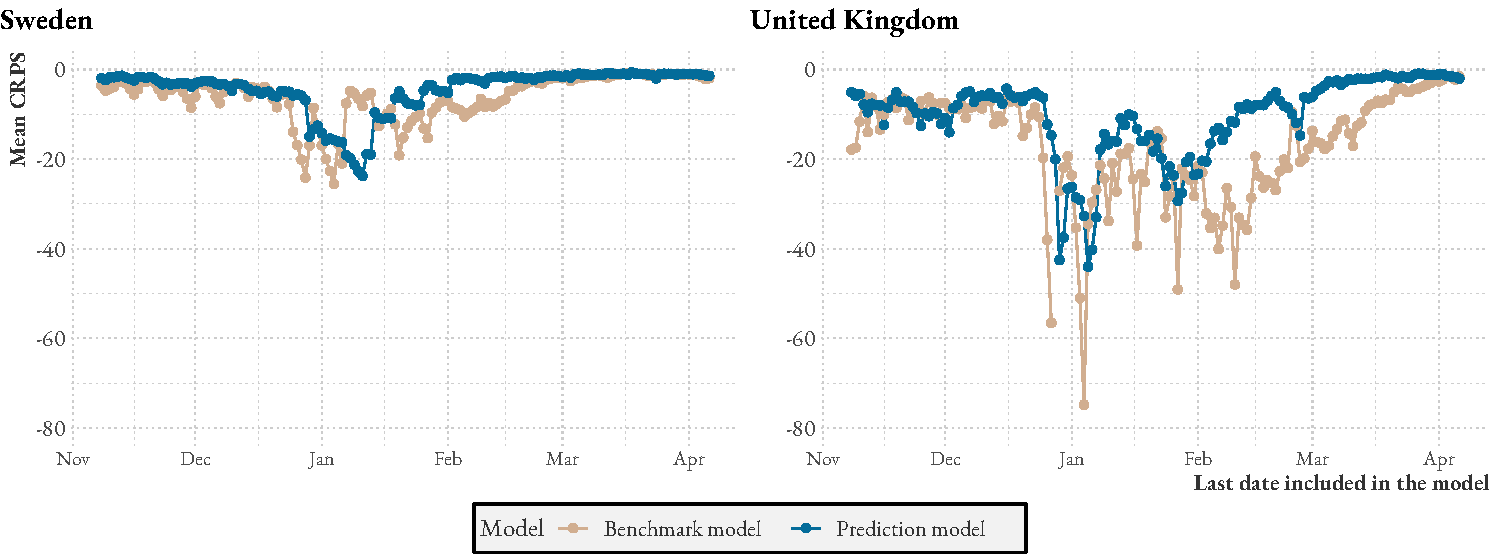
\includegraphics[width=0.9\textwidth]{plots/CRPS_over_states}
    \caption{Average SCRPS as the pandemic progresses.}
    \label{fig:SCRPS_states}
\end{figure}

\begin{figure}
    \centering
    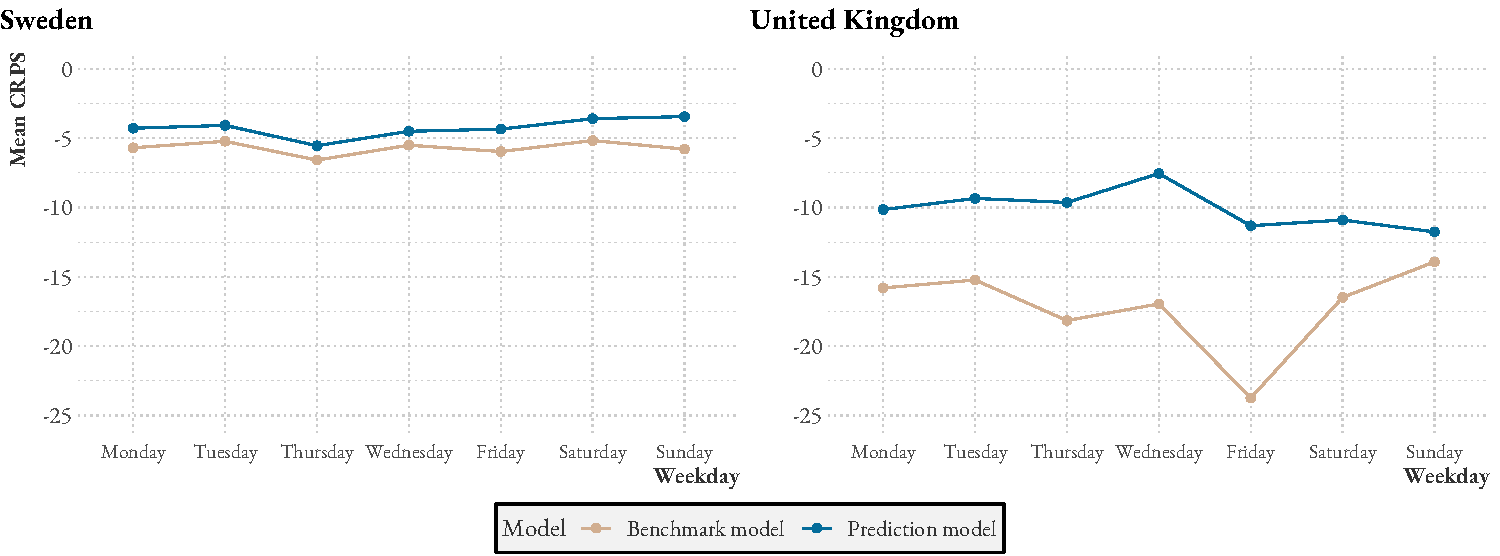
\includegraphics[width=0.9\textwidth]{plots/CRPS_over_weekdays}
    \caption{Average SCRPS per weekday.}
    \label{fig:SCRPS_weekdays}
\end{figure}%

\end{document}
